\documentclass[a4paper,12pt, oneside]{book}
%\pdfminorversion=5 
%\pdfcompresslevel=9
%\pdfobjcompresslevel=2
%\pdfminorversion=5
% \usepackage{fullpage}
\usepackage[italian]{babel}
\usepackage[utf8]{inputenc}
\usepackage[document]{ragged2e}
\usepackage{float}
\usepackage{amssymb}
\usepackage{graphicx}
\usepackage[font=small,labelfont=bf]{caption}
\usepackage{csquotes}
\usepackage{amsthm}
\usepackage{graphics}
\usepackage{amsfonts}
\usepackage{amsmath}
\usepackage{amstext}
\usepackage{engrec}
\usepackage{rotating}
\usepackage[safe,extra]{tipa}
\usepackage{tikz,pgfplots}
\usetikzlibrary{positioning}
\usetikzlibrary{calc,through,backgrounds}
\usepackage{stanli}
\usepackage{multirow}
\usepackage{titlesec}
\usepackage{hyperref}
\usepackage{microtype}
\usepackage{enumerate}
\usepackage{braket}
\usepackage{marginnote}
\usepackage{pgfplots}
\usepackage{cancel}
\usepackage{polynom}
\usepackage{caption}
\usepackage{booktabs}
\usepackage{enumitem}
\usepackage{framed}
\usepackage{pdfpages}
\usepackage{pdfpages}
\usepackage{pgfplots}
\usepackage{fancyhdr}
\fancyhead[LE,RO]{\slshape \rightmark}
\fancyhead[LO,RE]{\slshape \leftmark}
\fancyfoot[C]{\thepage}
\usepackage{endnotes}
\makeatletter
\makeatother
\renewcommand{\theendnote}{\Roman{endnote}} 
\renewcommand{\notesname}{Note}
\newenvironment{tightcenter}{%
	\setlength\topsep{0pt}
	\setlength\parskip{0pt}
	\begin{center}
	}{%
	\end{center}
}

\title{\textbf{Tecnica delle Costruzioni}\\ \textbf{Corso di laurea in ingegneria edile}\\ \textbf{Prof. Ing. Andrea Prota–a.a. 2022/2023}}
\author{Ivano D'Apice\\\\ N41002772}
\date{}

\pgfplotsset{compat=1.13}
\begin{document}
	\maketitle
	
	\definecolor{shadecolor}{gray}{0.80}
	
	\newtheorem{teorema}{Teorema}
	\newtheorem{definizione}{Definizione}
	\newtheorem{esempio}{Esempio}
	\newtheorem{corollario}{Corollario}
	\newtheorem{lemma}{Lemma}
	\newtheorem{osservazione}{Osservazione}
	\newtheorem{nota}{Nota}
	\newtheorem{esercizio}{Esercizio}
	\tableofcontents
	\renewcommand{\chaptermark}[1]{%
		\markboth{\chaptername
			\ \thechapter.\ #1}{}}
	\renewcommand{\sectionmark}[1]{\markright{\thesection.\ #1}}
	
	\chapter{Assegno Solaio}
	    
    \begin{tabbing}
	 Geometria \hspace{10em} \= \hspace{1em} \\
	 $L_1$=  $0,70+0,10\cdot n$              \> n=n.ro lettere del nome    \\
	 $L_2$=  $4,30+0,10\cdot c$              \> c=n.re lettere del cognome \\ 
	 $L_3$=  $4,80+0,10\cdot c-0,10\cdot n$  \>                             
    \end{tabbing}	    

	\begin{figure}[H]
		\centering
		\hspace*{-.5cm}
		\begin{tikzpicture}
			% here we construct our structure
			\scaling{.45};
			%\draw[help lines,step=.45]
			(0,-.9) grid (12.6,1.81);
			\point{a}{2}{1};                                
			\point{b}{26}{1};                               
			\point{c}{14}{1};                               
			\point{d}{0}{1};  
			\beam{2}{d}{b};                                          
			\support{1}{a}[0];                               
			\support{1}{b}[0];                               
			\support{1}{c}[0];        
			\dimensioning{1}{d}{a}{-1}[$L_1$];
			\dimensioning{1}{a}{c}{-1}[$L_2$];
			\dimensioning{1}{c}{b}{-1}[$L_3$];
			\notation{1}{d}{A}[below = 18mm];
			\notation{1}{a}{B}[below = 18mm];
			\notation{1}{c}{C}[below = 18mm];
			\notation{1}{b}{D}[below = 18mm];
		\end{tikzpicture}
		\caption{}
		\label{fig:travesolaio}
	\end{figure}
	
	\begin{figure}[H]
		\hspace*{-.4cm}
		\centering
		\includegraphics[width=0.7\linewidth]{"immagini/misure solaio flessione normale"}
		\caption{Dati numerici in 1 metro di solaio.}
		\label{fig:misure-solaio-flessione-normale}
	\end{figure}
	
	\begin{tabbing}
		Carichi Accidentali\endnote{I valori di carico accidentale in situazione normale sono $q=4.00kN/m^{2}$ e $q=2.00kN/m^{2}$ rispettivamente per lo sbalzo e campata. I valori usati in esercizio sono puramente didattici.} \hspace{10em} \= Matricola pari \hspace{1em} \\
		Sullo Sbalzo $\longrightarrow$    \> $Q_{k1}=5,00kN/m^{2}$    \\
		In Campata   $\longrightarrow$    \> $Q_{k2}=3,50kN/m^{2}$                     
	\end{tabbing}
	\chapter{Analisi dei carichi}
	
	Consideriamo due tipi di carico: $Q$ e $G$. I carichi di tipo $Q$ si dicono \textbf{variabili}, mentre quelli di tipo $G$ \textbf{permanenti}. Differenziamo poi i carichi $G$ in \textbf{permanenti strutturali} $G_1$ e \textbf{permanenti non strutturali} $G_2$.
    \leavevmode\newline
    \leavevmode\newline
	Si ricorda che verrà fatta una verifica rispetto allo \textbf{S.L.U} (Stati Limite Ultimo), tenendo conto dello \textbf{S.L.E} (Stato Limite di Esercizio) per quanto riguarda il dimensionamento del solaio.

	Dati:
	\begin{tabbing}
		\hspace{14em} \= \hspace{2em} \= \hspace{6em} \= \hspace{2em} \= \hspace{2em} \\ 
		$L_1$=  $0,70+0,10\cdot n$              \> = \> $0,70+0,50$ \> = \> $\textbf{1,20m}$  \\
		$L_2$=  $4,30+0,10\cdot c$              \> = \> $4,30+0,60$ \> = \> $\textbf{4,90m}$  \\
		$L_3$=  $4,80+0,10\cdot c-0,10\cdot n$  \> = \> $4,80+0,10$ \> = \> $\textbf{4,90m}$                     
	\end{tabbing}	
	\leavevmode\newline
	Utilizziamo la luce maggiore ($L_2=L_3$) per calcolare l'altezza del solaio grazie allo S.L.E. Avremo che $\textbf{H=}\frac{\textbf{L}}{\textbf{20}}$ e quindi $H=\frac{490cm}{20}=24,50cm\sim\textbf{25,00cm}$.
    \leavevmode\newline
    \leavevmode\newline
	Come da progetto [\ref{fig:misure-solaio-flessione-normale}] avremo $\textbf{H}_{sbalzo}=H-4,00cm=25,00cm-4,00cm=\textbf{21,00cm}$.\endnote{Considerando che una pignatta non è alta meno di 12 cm, l’altezza minima del solaio è comunque di 17 cm.}
	
	\break
	
	\section{Carichi strutturali permanenti $\textbf{G}_1$}
	
	\begin{tabbing}
		\textbf{Campata} \hspace{2em} \= \textbf{h} (m)\hspace{3em} \= \textbf{L} (m)\hspace{3em} \= $\textbf{P}$ (kN/m$^3$)\hspace{3em} \= $\textbf{G}_1$ (kN/m$^2$)\hspace{1em}\\\\
		Soletta  \> 0,05 \> 1,00           \> 25,00           \> 1,25  \\
		Travetti \> 0,20 \> 0,10$\cdot$2   \> 25,00           \> 1,00  \\ 
		Laterizi \endnote{Il peso specifico dei blocchi di allegerimento in laterizio è stato ricavato dalle tabelle dei pesi specifici di normativa, considerando una percentuale di foratura pari al 67\textdiscount (18$\cdot$[1-0,67]) = 5,94 -> 6,00 KN/m$^3$.} \> 0,20 \> 0,40$\cdot$2 \> \phantom{0}6,00 \> 	0,96                                    
	\end{tabbing}	    
	
	\begin{tabbing}
		\textbf{Sbalzo}\phantom{11.} \hspace{2em} \= \textbf{h} (m)\hspace{3em} \= \textbf{L} (m)\hspace{3em} \= $\textbf{P}$ (kN/m$^3$)\hspace{3em} \= $\textbf{G}_1$ (kN/m$^2$)\hspace{1em}\\\\
		Soletta  \> 0,05 \> 1,00           \> 25,00           \> 1,25  \\
		Travetti \> 0,16 \> 0,10$\cdot$2   \> 25,00           \> 0,80  \\ 
		Laterizi \> 0,16 \> 0,40$\cdot$2 \> \phantom{0}6,00   \> 0,77                                    
	\end{tabbing}

    \phantom{123}$\textbf{G}_{1campata}=(1,25+1,00+0,96)kN/m^2=3,21kN/m^2$ 
	
	\phantom{123}$\textbf{G}_{1sbalzo}\phantom{1.}=(1,25+0,80+0,77)kN/m^2=2,82kN/m^2$

    \section{Carichi permanenti non strutturali $\textbf{G}_2$}
    
    \begin{tabbing}
    	\phantom{\textbf{Campata}}\hspace{2em} \= \textbf{h} (m)\hspace{3em} \= \textbf{L} (m)\hspace{3em} \= $\textbf{P}$ (kN/m$^3$)\hspace{3em} \= $\textbf{G}_2$ (kN/m$^2$)\hspace{1em}\\\\
    	Massetto  \> 0,60 \> 1,00 \> 16,00           \> 0,96  \\
    	Pavimento \> 0,01 \> 1,00 \> 16,00           \> 0,18  \\ 
    	Intonaco  \> 0,01 \> 1,00 \> 18,00           \> 0,18                                    
    \end{tabbing}    
    
    Totale in campata e sullo sbalzo:\\
    \phantom{123}$\textbf{G}_2=(0,96+0,18+0,18)kN/m^2=1,32kN/m^2$ 
    
    \section{Condizioni di Carico}
    
    Dobbiamo usare i coefficienti parziali per le azioni nelle verifiche agli S.L.U per calcolare i carichi distribuiti da applicare al solaio.
    
    \begin{tabbing}
    	\phantom{Campata} \hspace{1em} \= \hspace{10em} \= \hspace{2em} \= \hspace{1em}\\\\
    	$G_{1campata}$    \> $3,21kN/m^2\cdot\gamma_{G1}$ \> = \> $4,17kN/m^2$ \\
    	$G_{1sbalzo}$     \> $2,82kN/m^2\cdot\gamma_{G1}$ \> = \> $3,67kN/m^2$ \\
    	$G_2$    \> $1,32kN/m^2\cdot\gamma_{G2}$ \> = \> $1,98kN/m^2$ \\ 
    	$Q_{k1}$ \> $5,00kN/m^2\cdot\gamma_{Q_{k1}}$ \endnote{In realtà bisogna comunque ricordare che essendo $Q_k$ un carico variabile, $\gamma_{Q1}$ può essere sia pari a 1,5, sia a 0. In questo caso sono stati riportati tutti i casi sfavorevoli.}\> = \> $7,50kN/m^2$ \\       
    	$Q_{k2}$ \> $3,50kN/m^2\cdot\gamma_{Q{k2}}$ \> = \> $5,25kN/m^2$                    
    \end{tabbing}	
    
    \chapter{Sollecitazioni di progetto allo Stato Limite Ultimo}
    
    I carichi permanenti $G_1, G_2$ e variabili $Q_k$, devono essere combinati tenendo conto dei coefficienti di sicurezza parziali ($\gamma_{G}$ e $\gamma_{Qk}$) in modo da ottenere le sollecitazioni più gravose allo S.L.U. Le condizioni di carico da considerare sono tre:
    \leavevmode\newline
    \leavevmode\newline
    \phantom{12}\textbf{1.} Entrambe le campate caricate con carichi permanenti e variabili, rispettivamente moltiplicati per i coefficienti parziali 1,30 e 1,50. Sullo sbalzo va considerato solo il carico permanente moltiplicato per il coefficiente parziale 1,30.
    \leavevmode\newline
    \phantom{12}\textbf{2.} Carichi permanenti su tutta la trave moltiplicati per il coefficiente parziale 1,30. Carichi variabili sulla prima campata e sullo sbalzo moltiplicati per il coefficiente parziale 1,50. 
    \leavevmode\newline
    \phantom{12}\textbf{3.} Carichi permanenti su tutta la trave moltiplicati per il coefficiente parziale 1,30. Carichi variabili solo sulla seconda campata, moltiplicati per il coefficiente parziale 1,50.
    
    \section{Combinazione di carico n° 1}
    
    \begin{figure}[H]
    	\centering
    	\hspace*{-1.9cm}
    	\begin{tikzpicture}
    		% here we construct our structure
    		\scaling{.45};
    		%\draw[help lines,step=.45]
    		(0,-.9) grid (12.6,1.81);
    		\point{a}{2}{1};                                
    		\point{b}{26}{1};                               
    		\point{c}{14}{1};                               
    		\point{d}{0}{1};
    		\point{caricovari}{2}{4};
    		\point{caricovarf}{26}{4};
    		\beam{2}{d}{b};                                          
    		\support{1}{a}[0];                               
    		\support{1}{b}[0];                               
    		\support{1}{c}[0];
    		\lineload{1}{caricovari}{caricovarf}[.569][.569][0.01];
    		\lineload{1}{a}{b}[1.088][1.088][.01];
    		\lineload{1}{d}{a}[1][1][.09];
    		\notation{1}{caricovarf}{$5,25kN/m$}[above right];
    		\notation{1}{b}{$6,15kN/m$}[above right];
    		\notation{1}{d}{$5,65kN/m$}[above left];
    	\end{tikzpicture}
    	\caption{}
    	\label{fig:travesolaiocarico1}
    \end{figure}

    Addizioniamo i carichi agenti sulle uguali campate.

    \begin{figure}[H]
    	\centering
    	\hspace*{-1.9cm}
    	\begin{tikzpicture}
    		% here we construct our structure
    		\scaling{.45};
    		%\draw[help lines,step=.45]
    		(0,-.9) grid (12.6,1.81);
    		\point{a}{2}{1};                                
    		\point{b}{26}{1};                               
    		\point{c}{14}{1};                               
    		\point{d}{0}{1};
    		\beam{2}{d}{b};                                          
    		\support{1}{a}[0];                               
    		\support{1}{b}[0];                               
    		\support{1}{c}[0];
    		\lineload{1}{a}{b}[1.657][1.657][.01];
    		\lineload{1}{d}{a}[1][1][.09];
    		\notation{1}{b}{$11,40kN/m$}[above right];
    		\notation{1}{d}{$5,65kN/m$}[above left];
    		\dimensioning{1}{d}{a}{-1.4}[$1,20$];
    		\dimensioning{1}{a}{c}{-1.4}[$4,90$];
    		\dimensioning{1}{c}{b}{-1.4}[$4,90$];
    	\end{tikzpicture}
    	\caption{}
    	\label{fig:travesolaiocaricouniformato1}
    \end{figure}

    \textbf{Metodo degli spostamenti:}
    \leavevmode\newline
    \leavevmode\newline
    $\boxtimes$ Come primo passaggio, possiamo semplificare lo sbalzo come un momento applicato all'estremo del vincolo in B.
    
    \begin{figure}[H]
    	\centering
    	\hspace*{-2cm}
    	\begin{tikzpicture}
    		% here we construct our structure
    		\scaling{.45};
    		%\draw[help lines,step=.45]
    		(0,-.9) grid (12.6,1.81);
    		\point{a}{2}{1};                                
    		\point{b}{26}{1};                               
    		\point{c}{14}{1}; 
    		\point{d}{.6}{1};                              
    		\beam{2}{a}{b};                                          
    		\support{1}{a}[0];                               
    		\support{1}{b}[0];                               
    		\support{1}{c}[0];
    		\load{3}{d}[90][180];
    		\lineload{1}{a}{b}[1.657][1.657][.01];
    		\notation{1}{b}{$11,40kN/m$}[above right];
    	    \notation{1}{d}{$4,07kNm$}[left=.5cm];
    	    \notation{1}{a}{B}[below=2cm];
    	    \notation{1}{b}{D}[below=2cm];
    	    \notation{1}{c}{C}[below=2cm];
    		\dimensioning{1}{a}{c}{-1.4}[$4,90$];
    		\dimensioning{1}{c}{b}{-1.4}[$4,90$];
    	\end{tikzpicture}
    	\caption{}
    	\label{fig:travesolaiocaricomomento}
    \end{figure}
    
    $\alpha$) \textbf{FASE A NODI BLOCCATI.} 
    \leavevmode\newline
    \leavevmode\newline
    $\boxtimes$ Aggiungiamo un vincolo fittizio (morsetto) in mezzeria.
    
    \begin{figure}[H]
    	\centering
    	\hspace*{-1.5cm}
    	\begin{tikzpicture}
    		% here we construct our structure
    		\scaling{.45};
    		%\draw[help lines,step=.45]
    		(0,-.9) grid (12.6,1.81);
    		\point{a}{2}{1};                                
    		\point{b}{26}{1};                               
    		\point{c}{14}{1}; 
    		\point{d}{.6}{1};                              
    		\beam{2}{a}{b};                                          
    		\support{1}{a}[0];                               
    		\support{1}{b}[0];                               
    		\support{1}{c}[0];
    		\load{3}{d}[90][180];
    		\lineload{1}{a}{b}[1.657][1.657][.01];
    		\notation{1}{b}{$11,40kN/m$}[above right];
    		\notation{1}{d}{$4,07kNm$}[left=.5cm];
    		\notation{1}{c}{$\bullet$}[above left=-1.3mm];
    		\notation{1}{c}{$\bullet$}[above right=-1.3mm];
    		\notation{1}{c}{$\bullet$}[below left=-1.3mm];
    		\notation{1}{c}{$\bullet$}[below right=-1.3mm];
    	\end{tikzpicture}
    	\caption{}
    	\label{fig:travesolaiocaricfitt}
    \end{figure}

    \begin{figure}[H]
    	\centering
    	\hspace*{-1.5cm}
    	\begin{tikzpicture}
    		\centering
    		% here we construct our structure
    		\scaling{.45};
    		%\draw[help lines,step=.45]
    		(0,-.9) grid (12.6,1.81);
    		\point{a}{2}{1};                                 %Punto A
    		\point{b}{26}{1};                                %Punto B
    		\point{c}{14}{1};                                %Punto C
    		\point{d}{.6}{1}
    		\point{e}{27}{1};
    		\beam{2}{a}{b};                                  %Trave A-B
    		\support{1}{a}[0];                               %Cerniera A
    		\support{3}{b}[90];                               %Carrello B
    		\load{3}{d}[90][180];
    		\load{3}{e}[270][180];
    		\notation{1}{d}{$4,07kNm$}[left=.5cm];
    		\notation{1}{e}{$\frac{4,07kNm\endnote{Quando abbiamo un incastro-appoggio con una coppia esterna, la coppia opposta andrà dimezzata}}{2}$}[right=.5cm];
    	\end{tikzpicture}
    	\caption{Tratto BC.}
    	\label{fig:trattobcmomento}
    \end{figure}

    \begin{tightcenter}
    $M_{c}^{sx}(M_b)=-2,04kNm$
    \end{tightcenter}

    \leavevmode\newline
    \begin{figure}[H]
    	\centering
    	\hspace*{-.3cm}
    	\begin{tikzpicture}
    		\centering
    		% here we construct our structure
    		\scaling{.45};
    		%\draw[help lines,step=.45]
    		(0,-.9) grid (12.6,1.81);
    		\point{a}{2}{1};                                 %Punto A
    		\point{b}{26}{1};                                %Punto B
    		\point{c}{14}{1};                                %Punto C
    		\point{d}{.6}{1}
    		\point{e}{27}{1};
    		\point{f}{2}{1.8};
    		\point{g}{26}{1.8};
    		\beam{2}{a}{b};                                  %Trave A-B
    		\support{1}{a}[0];                               %Cerniera A
    		\support{3}{b}[90];                              %Carrello B
    		\load{3}{d}[90][180];
    		\load{2}{e}[270][180];
    		\lineload{1}{f}{g}[1][1][0.01];
    		\notation{1}{d}{$\frac{qL^{2}}{8}$}[left=.5cm];
    		\notation{1}{e}{$34,21kNm$}[right=.5cm];
    	\end{tikzpicture}
    	\caption{Tratto BC.}
    	\label{fig:trattobccarico}
    \end{figure}

    \begin{tightcenter}
    $M_{c}^{sx}(q)=34,21kNm$
    \end{tightcenter}
    
    \leavevmode\newline
    \begin{figure}[H]
    	\centering
    	\hspace*{-1.7cm}
    	\begin{tikzpicture}
    		\centering
    		% here we construct our structure
    		\scaling{.45};
    		%\draw[help lines,step=.45]
    		(0,-.9) grid (12.6,1.81);
    		\point{a}{2}{1};                                 %Punto A
    		\point{b}{26}{1};                                %Punto B
    		\point{c}{14}{1};                                %Punto C
    		\point{d}{.6}{1}
    		\point{e}{27}{1};
    		\point{f}{2}{1.8};
    		\point{g}{26}{1.8};
    		\beam{2}{a}{b};    
    		\support{3}{a}[-90];                            
    		\support{1}{b};                               %Carrello B
    		\load{3}{d}[90][180];
    		\load{2}{e}[270][180];
    		\lineload{1}{f}{g}[1][1][0.01];
    		\notation{1}{e}{$\frac{qL^{2}}{8}$}[right=.5cm];
    		\notation{1}{d}{$34,21kNm$}[left=.5cm];
    	\end{tikzpicture}
    	\caption{Tratto CD.}
    	\label{fig:trattocdcarico}
    \end{figure}

    \begin{tightcenter}
    $M_{c}^{dx}(q)=-34,21kNm$
    \end{tightcenter}
    
    \leavevmode\newline
    \leavevmode\newline
    \leavevmode\newline
    $\beta$) \textbf{ATTIVAZIONE DEGLI SPOSTAMENTI NODALI.} $\hfill$

    \begin{figure}[H]
    	\centering
    	\hspace*{.2cm}
    	\begin{tikzpicture}
    		% here we construct our structure
    		\scaling{.45};
    		%\draw[help lines,step=.45]
    		(0,-.9) grid (12.6,1.81);
    		\point{a}{2}{1};               				
    		\point{b}{14}{1};             				
    		\point{c}{26}{1};
    		\point{d}{2}{-4};
    		\point{e}{14}{-4};
    		\point{f}{26}{-4};
    		\point{g}{1.4}{3};
    		\point{h}{26.6}{3};
    		\beam{2}{a}{c};
    		\support{1}{a}[0];
    		\support{1}{b}[0];
    		\support{1}{c}[0];
    		\internalforces{a}{b}{0}{0}[1][gray];
    		\internalforces{b}{c}{0}{0}[-1][gray];
    		\notation{1}{b}{$\bullet$}[above left=-1.3mm];
    		\notation{1}{b}{$\bullet$}[above right=-1.3mm];
    		\notation{1}{b}{$\bullet$}[below left=-1.3mm];
    		\notation{1}{b}{$\bullet$}[below right=-1.3mm];
    	\end{tikzpicture}
    	\caption{Flessione dei tronchi indotta dagli spostamenti.}
    	\label{fig:spostamentonodale}
    \end{figure}

    \begin{figure}[H]
    	\centering
    	\hspace*{.8cm}
    	\begin{tikzpicture}
    		% here we construct our structure
    		\scaling{.45};
    		%\draw[help lines,step=.45]
    		(0,-.9) grid (12.6,1.81);
    		\point{a}{2}{1};               				             				
    		\point{b}{26}{1};
    		\point{c}{27}{1};
    		\beam{2}{a}{b};
    		\support{1}{a}[0];
    		\support{3}{b}[90];
    		\load{2}{c}[270][180];
    		\internalforces{a}{b}{0}{0}[1][gray];
    		\notation{1}{c}{$\frac{3EI}{L_2}\varphi_{c}$}[right=.5cm];
    	\end{tikzpicture}
    	\caption{Tratto BC.}
    	\label{fig:spostamentonodalebc}
    \end{figure}

    \begin{tightcenter}
    $M_{c}^{sx}(\varphi_{c})=\frac{3EI}{4,90m}\varphi_{c}$
    \end{tightcenter}
    
    \begin{figure}[H]
    	\centering
    	\hspace*{-1.4cm}
    	\begin{tikzpicture}
    		% here we construct our structure
    		\scaling{.45};
    		%\draw[help lines,step=.45]
    		(0,-.9) grid (12.6,1.81);
    		\point{a}{2}{1};               				             				
    		\point{b}{26}{1};
    		\point{c}{1}{1};
    		\beam{2}{a}{b};
    		\support{3}{a}[-90];
    		\support{1}{b}[0];
    		\load{2}{c}[90][180];
    		\internalforces{a}{b}{0}{0}[-1][gray];
    		\notation{1}{c}{$\frac{3EI}{L_3}\varphi_{c}$}[left=.5cm];
    	\end{tikzpicture}
    	\caption{Tratto CD.}
    	\label{fig:spostamentonodalecd}
    \end{figure}

    \begin{tightcenter}
    $M_{c}^{dx}(\varphi_{c})=\frac{3EI}{4,90m}\varphi_{c}$
    \end{tightcenter}
    \leavevmode\newline
    \leavevmode\newline
    \leavevmode\newline
    $\gamma$) \textbf{SCRITTURA DELL'EQUAZIONE DI EQUILIBRIO AL NODO.} 
    \leavevmode\newline
    \leavevmode\newline
    \begin{tightcenter}
      $ M_{csx}+M_{cdx}-M_{est}=0  $
    \end{tightcenter}
    \leavevmode\newline 
    \begin{equation}
    	\begin{cases}
    		M_{c}^{sx}(M_b)+M_{c}^{sx}(q)+M_{c}^{sx}(\varphi_{c})+M_{c}^{dx}(q)+M_{c}^{dx}(\varphi_{c})&=0 \\ \\
    		-2,04kNm+34,21kNm+\frac{3EI}{4,90m}\varphi_{c}-34,21kNm+\frac{3EI}{4,90m}\varphi_{c}&=0\\ \\ 
    	\end{cases}
    	\hfill
    \end{equation}
   \leavevmode\newline
    \begin{equation}
    	\begin{cases}
    		\varphi_{c}&=\frac{10,00kNm^{2}}{6EI}\\ \\
    		M_{c}^{sx}=M_{c}^{dx}(\varphi_{c})=\frac{3EI}{4,90m}\cdot\frac{10,00kNm^{2}}{6EI}=\frac{10,00kNm^{2}}{4,90m}\frac{3EI}{6EI}&=1,02kNm\\ \\ 
    	\end{cases}
    	\hfill
    \end{equation}
    \leavevmode\newline
    \begin{equation}
    	\begin{cases}
    		M_{CB}=2,04kNm-34,21kNm-1,02kNm\phantom{tes}&=-33,19kNm \\ \\
    		M_{CD}=-34,21kNm+1,02kNm\phantom{tes}&=-33,19kNm\\ \\ 
    	\end{cases}
    	\hfill
    \end{equation}
    \leavevmode\newline
    \leavevmode\newline
    \leavevmode\newline
    \leavevmode\newline
    $\delta$) \textbf{REAZIONI VINCOLARI.}
    \leavevmode\newline
    \leavevmode\newline
    \begin{figure}[H]
    	\centering
    	\hspace*{-1.6cm}
    	\begin{tikzpicture}
    		\centering
    		% here we construct our structure
    		\scaling{.45};
    		%\draw[help lines,step=.45]
    		(0,-.9) grid (12.6,1.81);
    		\point{a}{2}{1};                                 %Punto A
    		\point{b}{26}{1};                                %Punto B
    		\point{c}{14}{1};                                %Punto C
    		\point{d}{.6}{1}
    		\point{e}{27}{1};
    		\point{f}{2}{1.8};
    		\point{g}{26}{1.8};
    		\point{ccccc}{2}{-1};
    		\point{bbbbb}{26}{-1};
    		\beam{2}{a}{b};                                  %Trave A-B
    		\support{1}{a}[0];                               %Cerniera A
    		\support{1}{b}[0];                              %Carrello B
    		\load{3}{d}[90][180];
    		\load{2}{e}[270][180];
    		\load{1}{c}[90];
    		\load{1}{a}[-90][1][1];
    		\load{1}{b}[-90][1][1];
       		\notation{1}{d}{$4,07kNm$}[left=.5cm];
    		\notation{1}{e}{$33,19kNm$}[right=.5cm];
    		\notation{1}{c}{$55,86kN$}[above right=3mm];
    		\notation{1}{ccccc}{$R_b$}[below right=4mm];
    		\notation{1}{bbbbb}{$R_{c}^{sx}$}[below left=4mm];
    	\end{tikzpicture}
    	\caption{Tratto BC.}
    	\label{fig:reazionevincolareBC}
    \end{figure}
    
    \begin{alignat*}{5}
    	\Sigma Y\phantom{_b}   & {}=0{} & \phantom{123456} & R_b+R_{c}^{sx}-55,86kN       & {}=0{}\\
    	\Sigma M_b & {}=0{} & \phantom{123456} & \frac{55,86kN\cdot4,90m}{2}-R_{c}^{sx}\cdot4,90m+33,19kNm-4,07kNm & {}=0{} 
    \end{alignat*}
    \leavevmode\newline
    \leavevmode\newline
    $R_{c}^{sx}\cdot\phantom{,}4,90m=136,86kNm+29,12kNm$
    \leavevmode\newline
    \leavevmode\newline
    $R_{c}^{sx}=\frac{165,98kNm}{4,90m}=33,87kN$
    \leavevmode\newline
    \leavevmode\newline
    $R_b=55,86kN-33,87kN=21,99kN$
    
    \begin{figure}[H]
    	\centering
    	\hspace*{-1.6cm}
    	\begin{tikzpicture}
    		\centering
    		% here we construct our structure
    		\scaling{.45};
    		%\draw[help lines,step=.45]
    		(0,-.9) grid (12.6,1.81);
    		\point{a}{2}{1};                                 %Punto A
    		\point{b}{26}{1};                                %Punto B
    		\point{c}{14}{1};                                %Punto C
    		\point{d}{.6}{1}
    		\point{e}{27}{1};
    		\point{f}{2}{1.8};
    		\point{g}{26}{1.8};
    		\point{ccccc}{2}{-1};
    		\point{bbbbb}{26}{-1};
    		\beam{2}{a}{b};                                  %Trave A-B
    		\support{1}{a}[0];                               %Cerniera A
    		\support{1}{b}[0];                              %Carrello B
    		\load{3}{d}[90][180];
    		\load{1}{c}[90];
    		\load{1}{a}[-90][1][1];
    		\load{1}{b}[-90][1][1];
    		\notation{1}{d}{$33,19kNm$}[left=.5cm];
    		\notation{1}{c}{$55,86kN$}[above right=3mm];
    		\notation{1}{ccccc}{$R_{c}^{dx}$}[below right=4mm];
    		\notation{1}{bbbbb}{$R_d$}[below left=4mm];
    	\end{tikzpicture}
    	\caption{Tratto CD.}
    	\label{fig:reazionevincolareCD}
    \end{figure}

    \begin{alignat*}{5}
    	\Sigma Y\phantom{_b}   & {}=0{} & \phantom{123456} & R_{c}^{dx}+R_d-55,86kN & {}=0{}\\
    	\Sigma M_c & {}=0{} & \phantom{123456} & 136,86kNm-R_d\cdot4,90m-33,19kNm& {}=0{} 
    \end{alignat*}
    \leavevmode\newline
    \leavevmode\newline
    $R_d\cdot\phantom{,}4,90m=103,67kNm$
    \leavevmode\newline
    \leavevmode\newline
    $R_d=\frac{103,67kNm}{4,90m}=21,16kN$
    \leavevmode\newline
    \leavevmode\newline
    $R_{c}^{dx}=55,86kN-21,16kN=34,70kN$
    \leavevmode\newline
    \leavevmode\newline
    \leavevmode\newline
    \leavevmode\newline
    \leavevmode\newline
    $\textbf{R}_b=21,99kN,\leavevmode\newline\leavevmode\newline \textbf{R}_{c}^{sx}=33,87kN,\leavevmode\newline\leavevmode\newline \textbf{R}_{c}^{dx}=34,70kN,\leavevmode\newline\leavevmode\newline \textbf{R}_d=21,16kN\leavevmode\newline$
    
    \break
    
    $\pi$) \textbf{EQUAZIONI TAGLIO E MOMENTO.}
    \leavevmode\newline
    \leavevmode\newline
    \phantom{testoabcdefgh}{\tiny TRATTO B-C}
    \begin{equation}
    	\begin{cases}
    	T(x)&=R_b-q\cdot x \\ \\
        M(x)&=R_b\cdot x-M_b-\frac{q\cdot x^2}{2}\\ \\ 
    	\end{cases}
    	\hfill
    \end{equation}

    \phantom{testoabcdefgh}{\tiny TRATTO C-D}
    \begin{equation}
    	\begin{cases}
    		T(x)&=R_{c}^{dx}-q\cdot x \\ \\
    		M(x)&=R_{c}^{dx}\cdot x-M_c-\frac{q\cdot x^2}{2}\\ \\ 
    	\end{cases}
    	\hfill
    \end{equation}
    \leavevmode\newline
    \leavevmode\newline
    \leavevmode\newline
    \phantom{tes}{\tiny TRATTO B-C}
    \begin{equation}
    	\begin{cases}
    		T(0)&=\textbf{21,99kN} \\ \\
    		M(0)&=\textbf{-4,07kNm}\\ \\ 
    		T(4,90m)&=21,99kN-55,86kN=\textbf{-33,87kN}\\ \\ 
    		M(4,90m)&=-4,07kNm+107,75kNm-136,86kNm=\textbf{-33,19kNm}\\ \\ 
    		M(2,45m)&=-4,07kNm+53,88kNm-34,21kNm=\textbf{15,60kNm}
    	\end{cases}
    	\hfill
    \end{equation}
    
    \phantom{tes}{\tiny TRATTO C-D}
    \begin{equation}
    	\begin{cases}
    		T(0)&=\textbf{34,70kN} \\ \\
    		M(0)&=\textbf{-33,19kNm}\\ \\ 
    		T(4,90m)&=34,70kN-55,86kN=\textbf{-21,16kN}\\ \\ 
    		M(4,90m)&=-33,19kNm+170,03kNm-136,86kNm=\textbf{0,0kNm}\\ \\ 
    		M(2,45m)&=-33,19kNm+85,02kNm-34,21kNm=\textbf{17,62kNm}
    	\end{cases}
    	\hfill
    \end{equation}
    
    \begin{figure}[H]
    	\centering
    	\begin{tikzpicture}
    		% here we construct our structure
    		\scaling{.45};
    		%\draw[help lines,step=.45]
    		(0,-.9) grid (12.6,1.81);                              
    		\point{a}{0}{1};
    		\point{b}{2}{1}; 
    		\point{c}{14}{1}; 
    		\point{d}{26}{1};
    		\beam{2}{a}{d};                                          
    		\support{1}{b}[0];                               
    		\support{1}{c}[0];                               
    		\support{1}{d}[0];
    		\internalforces{a}{b}{0}{0.678}[0][blue][0];
    		\internalforces{b}{c}{-1.877}{2.582}[0][blue][0];
    		\internalforces{c}{d}{-2.935}{1.794}[0][blue][0];
    	\end{tikzpicture}
    	\caption{}
    	\label{fig:taglio}
    \end{figure}
   
    \begin{figure}[H]
    	\centering	
    	\begin{tikzpicture}
    		% here we construct our structure
    		\scaling{.45};
    		%\draw[help lines,step=.45]
    		(0,-.9) grid (12.6,1.81);                              
    		\point{a}{0}{1};
    		\point{b}{2}{1}; 
    		\point{c}{14}{1}; 
    		\point{d}{26}{1};
    		\point{e}{6}{1};
    		\beam{2}{a}{d};                                          
    		\support{1}{b}[0];                               
    		\support{1}{c}[0];                               
    		\support{1}{d}[0];
    		\internalforces{b}{c}{-0.407}{-2.794}[-1.296][blue][1];
    		\internalforces{c}{d}{-2.794}{0}[-1.501][blue][1];
    		\internalforces{a}{b}{0}{-0.407}[0.0001][blue][1];
    	\end{tikzpicture}
    	\caption{}
    	\label{fig:momento}
    \end{figure}
    
    \section{Combinazione di carico n° 2}
    
    \begin{figure}[H]
    \hspace*{-3.7cm}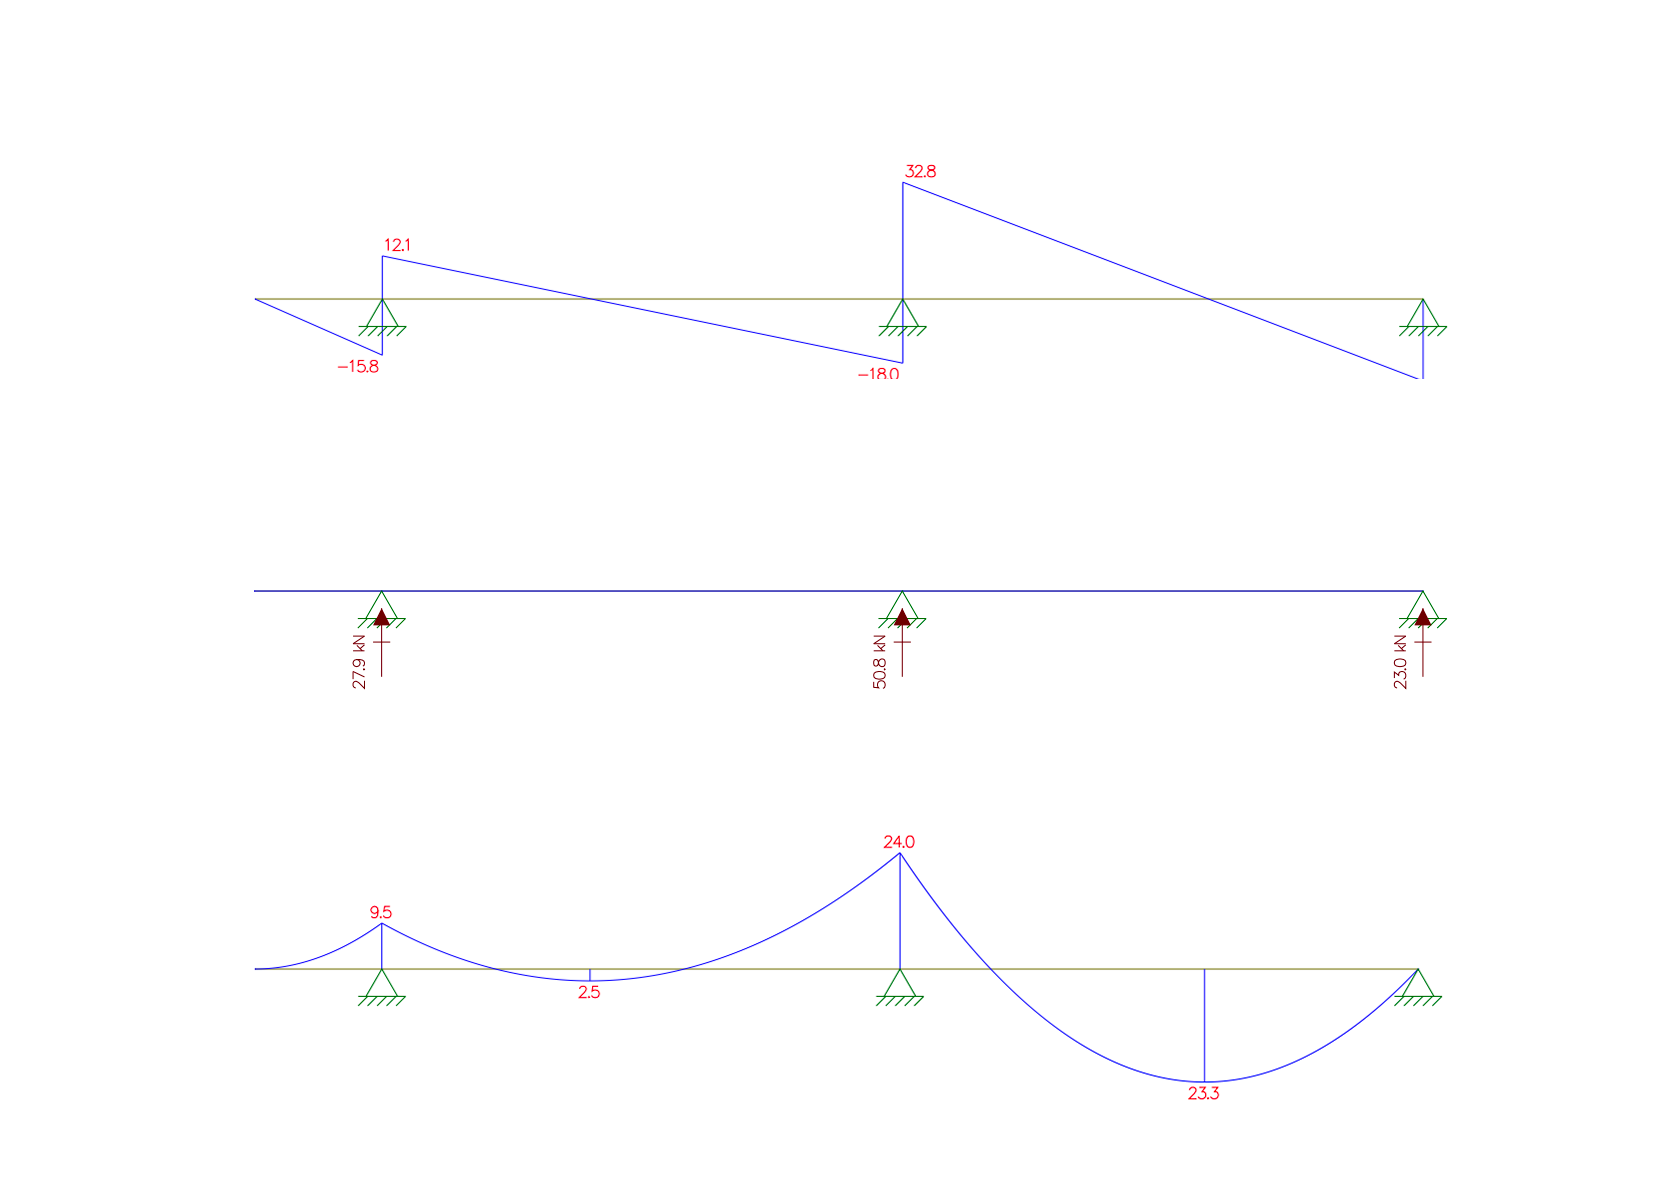
\includegraphics[width=1.5\linewidth]{"immagini/caso 2.png"}
    \end{figure}
    
    \break
    
    \section{Combinazione di carico n° 3}

    \begin{figure}[H]
    	\hspace*{-3.cm}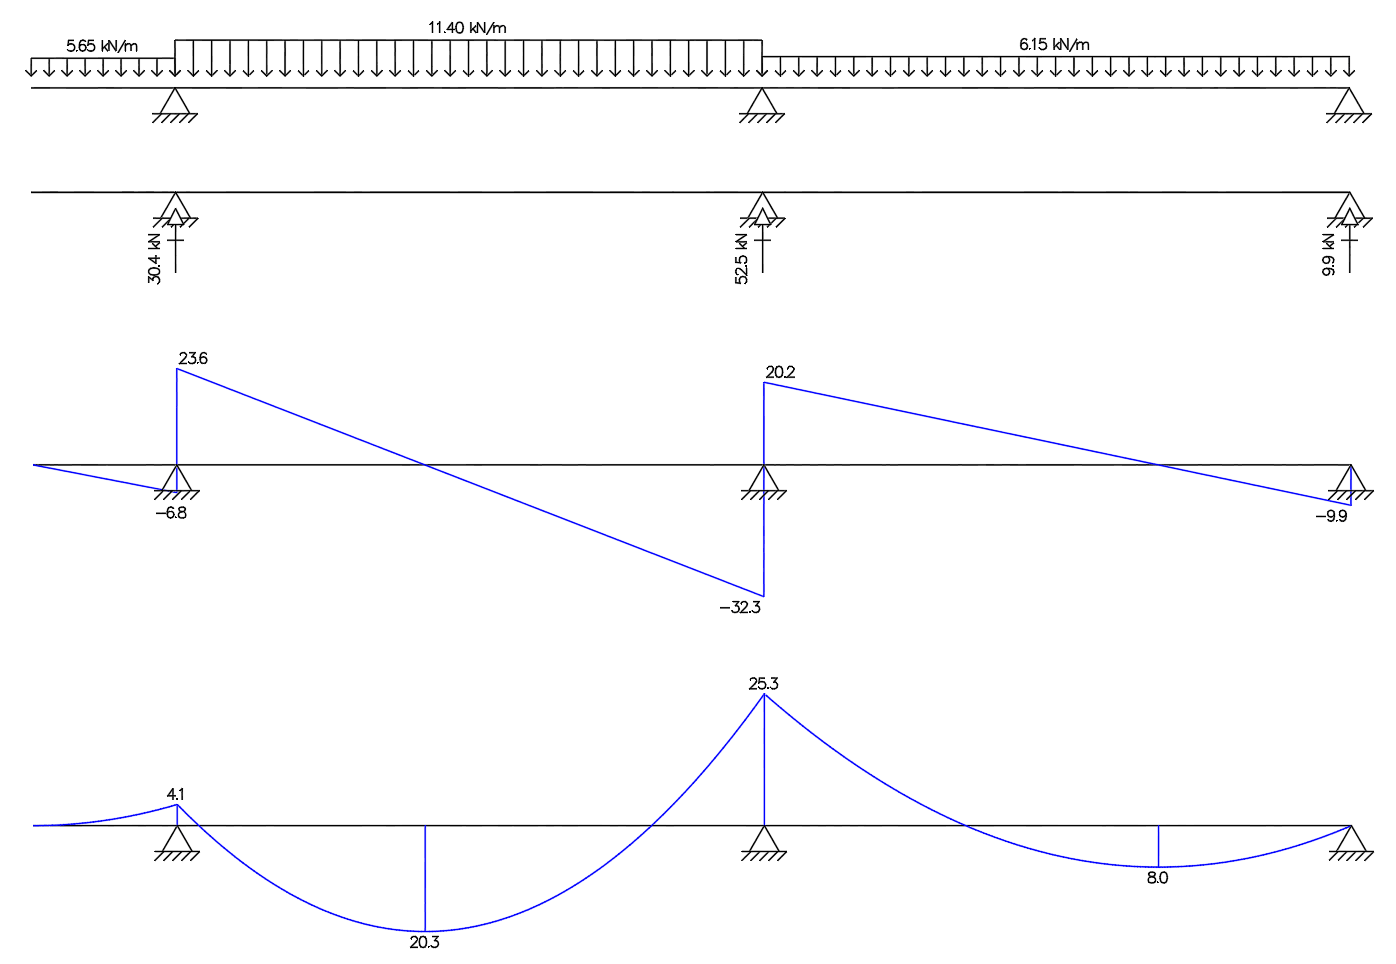
\includegraphics[width=1.4\linewidth]{"immagini/caso 3.png"}
    \end{figure}

    \section{Inviluppo momenti}

    \begin{figure}[H]
    	\hspace*{-2.8cm}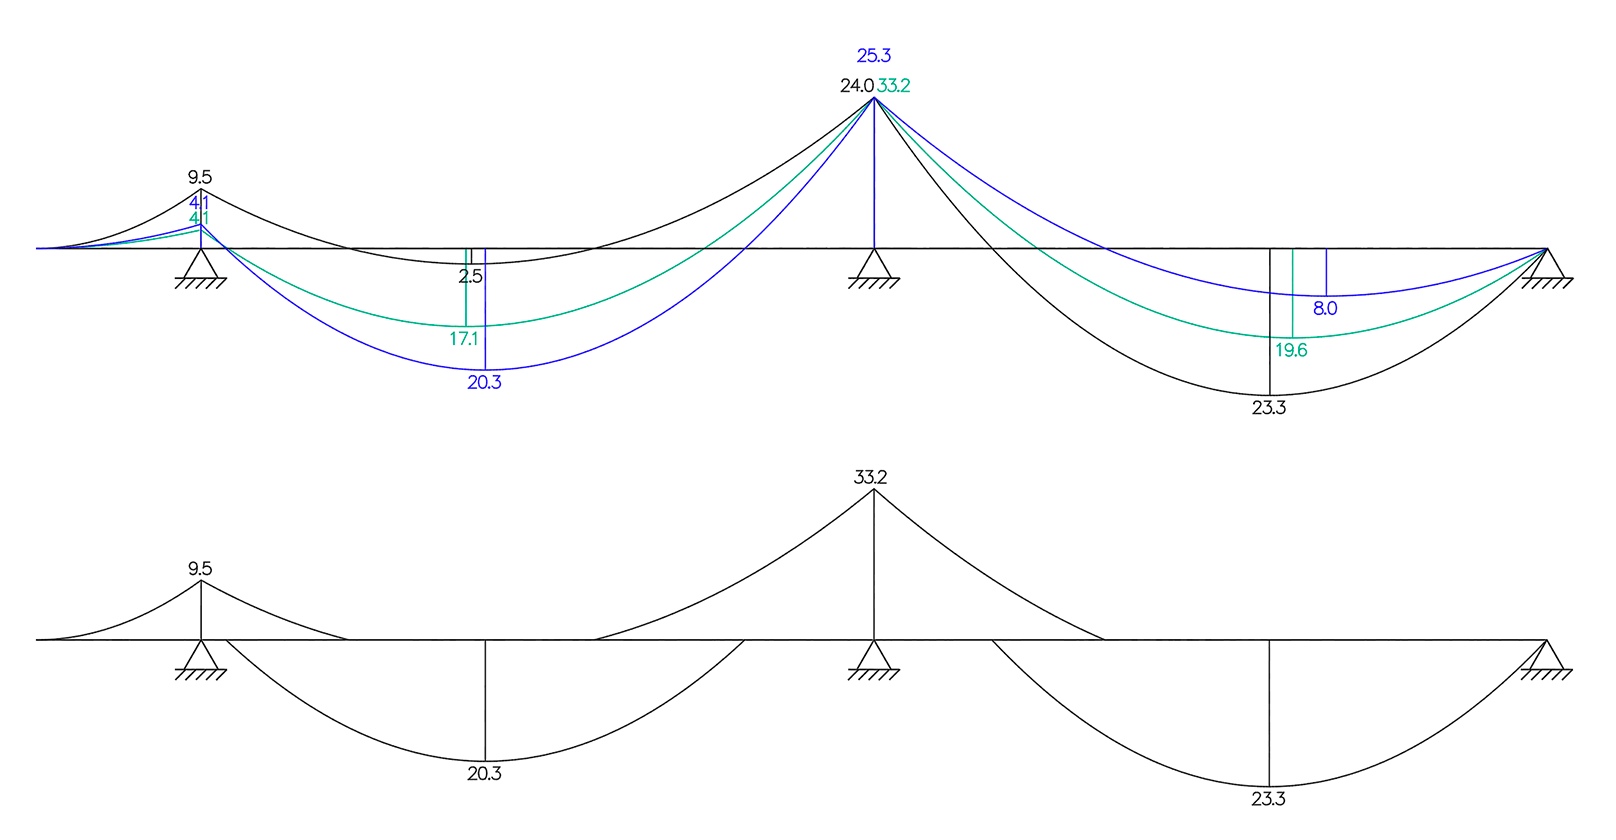
\includegraphics[width=1.4\linewidth]{"immagini/inviluppo momenti.png"}
    \end{figure}


	\newpage
	\begingroup
	\parindent 0pt
	\parskip 2ex
	\def\enotesize{\normalsize}
	\theendnotes
	\endgroup

\end{document}